\section{Results}

For the evaluation of the segmentation, as proposed in the
project statement, leave-one-out has been used. In this technique,
the data of the tooth we are trying to locate and segmentate is left
out of the trainign set, and it is used to test the obtained result.

But we need to know how good we have segmentated a given tooth with
respect to the ground truth. For this, the Jaccard index has been used.
The Jaccard Index or Jaccard coefficient is a statistic used for
comparing the similarity and diversity of
sample sets. The Jaccard coefficient measures similarity between
finite sample sets, and is defined as the size of the intersection
divided by the size of the union of the sample sets.

$$ J(A,B) =  \frac{|A \cap B|}{|A \cup B|} = \frac{|A \cap B|}{|A| + |B| - |A \cap B|} $$

The result will be a number between 0 (no overlap) and
1 (perfect segmentation).

 \begin{figure} \centering
  \frame{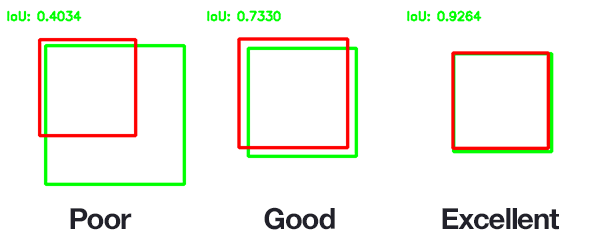
\includegraphics[width=0.6\linewidth]{img/iou}}
  \caption{Index of Union}
\end{figure}

\subsection{Manual initialization}

\begin{figure}[!htb] \centering
  \begin{minipage}{0.49\textwidth}
  \frame{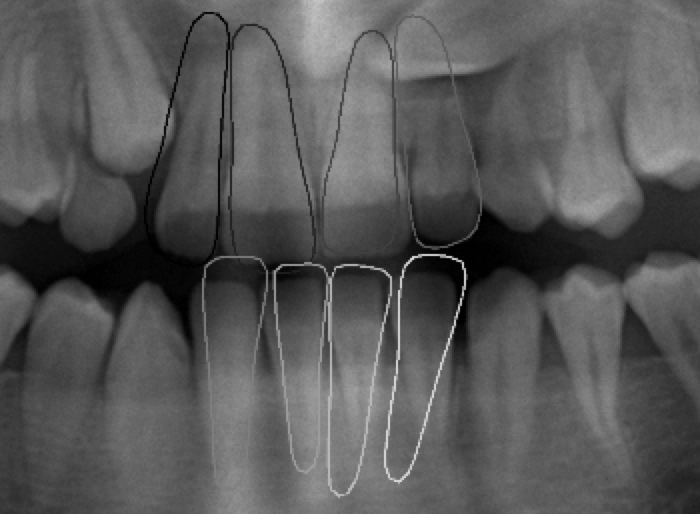
\includegraphics[width=\linewidth]{img/manual}}
  \caption{Result (manual initialization)}
\end{minipage}
\begin{minipage}{0.49\textwidth} \centering
  \frame{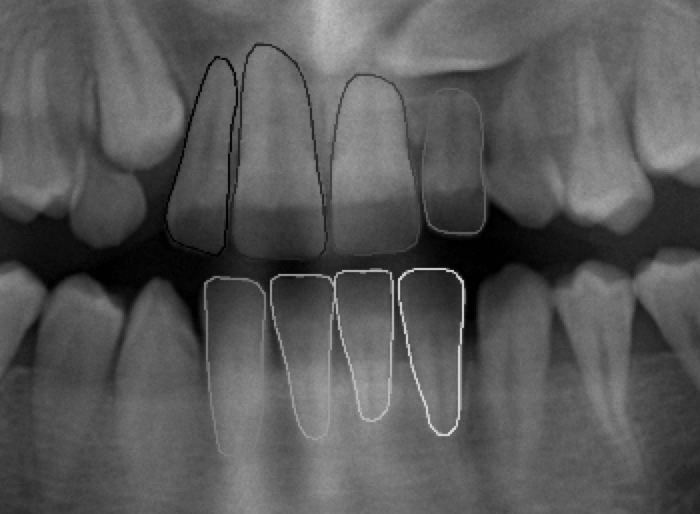
\includegraphics[width=\linewidth]{img/manual_truth}}
  \caption{Ground truth}
 \end{minipage}
\end{figure}

It can be seen that, in general, the crown of each tooth is
approximated well, but the root is not. This is caused by how
the fitting is done. As we use Grey Level Models, in the enhanced
images the contour of the tooth is much more defined in the crown.

 \begin{figure} \centering
  \frame{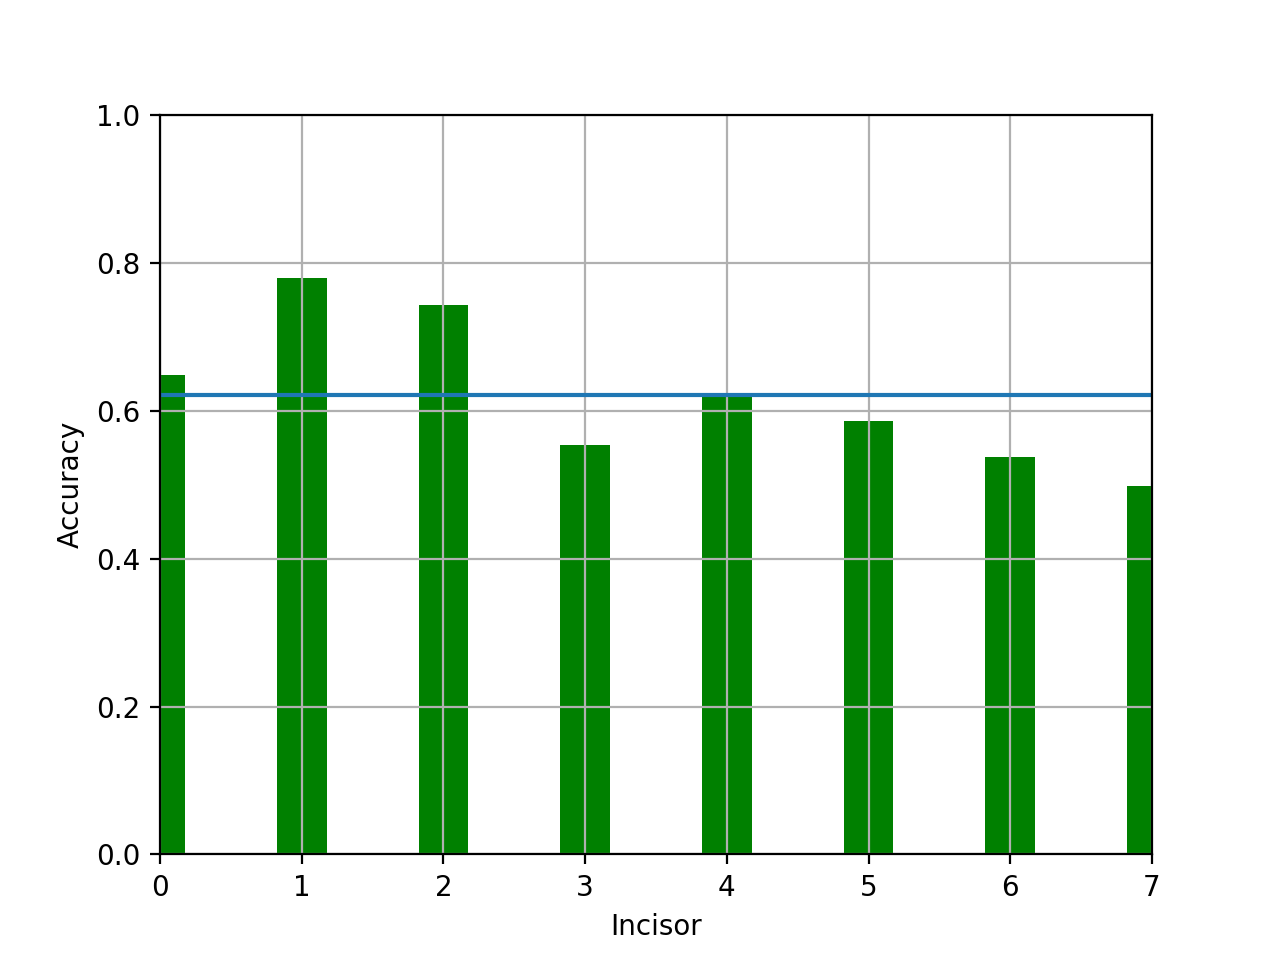
\includegraphics[width=0.6\linewidth]{img/acc_manual}}
  \caption{Accuracy of the segmentation}
\end{figure}


\subsection{Automatic initialization}
% TODO
 \begin{figure} \centering
  \frame{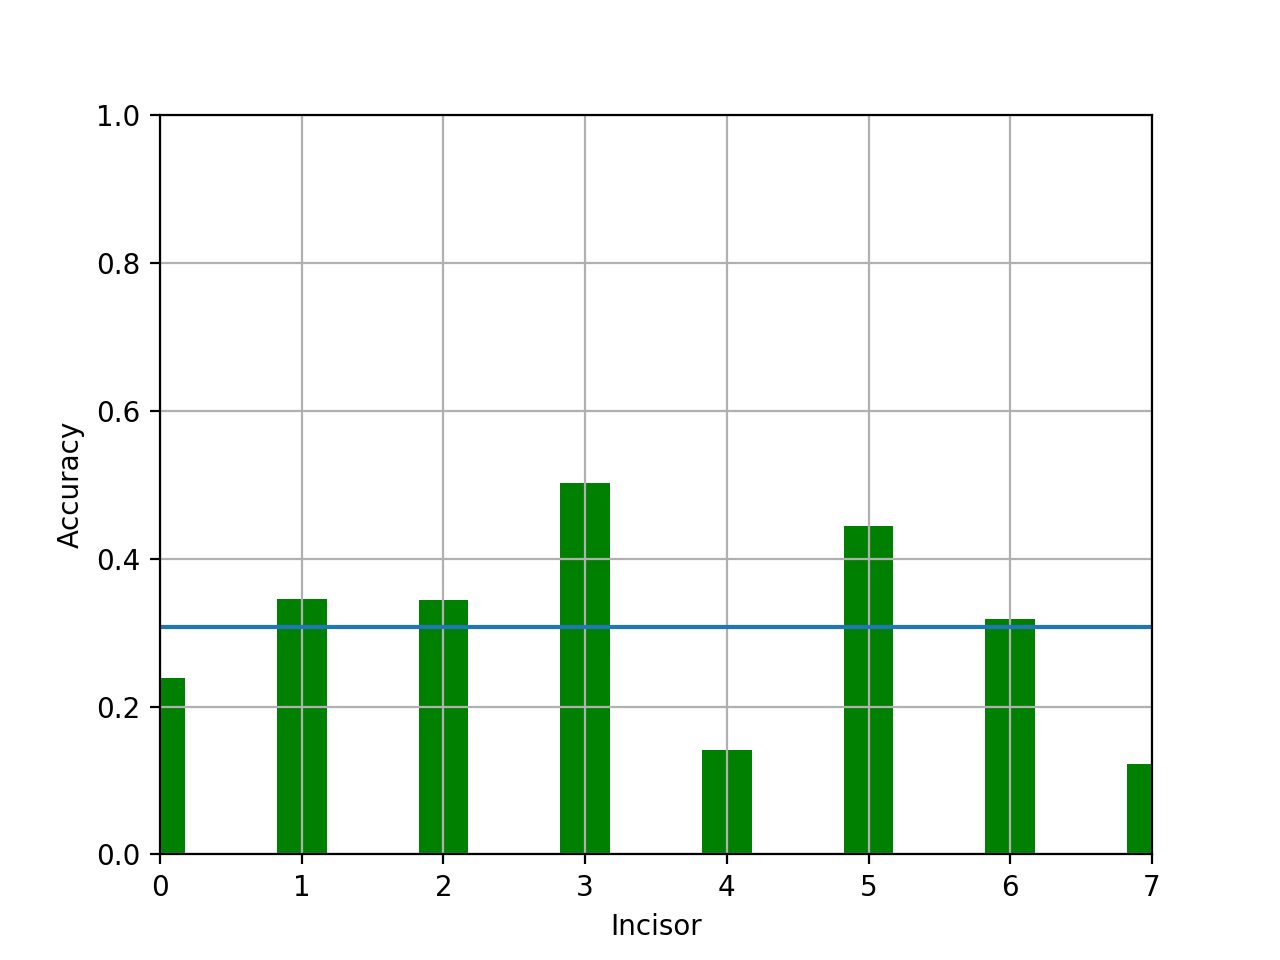
\includegraphics[width=0.6\linewidth]{img/acc_auto}}
  \caption{Accuracy of the segmentation}
\end{figure}


 \begin{figure} \centering
  \frame{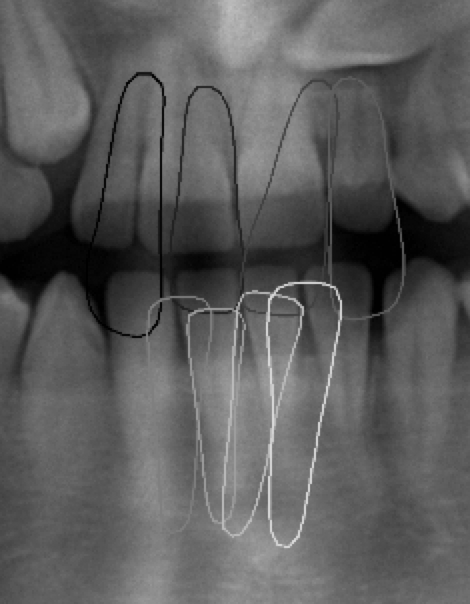
\includegraphics[width=0.6\linewidth]{img/auto}}
  \caption{Result (automatic initialization)}
\end{figure}



